\documentclass[12pt,oneside,letterpaper,english]{article}

\usepackage{Settings}

\begin{document}
\pagenumbering{roman} 

\begin{titlepage}
\begin{center}
\vspace{1 cm}
%\textsc{University of Bridgeport}\\[1.5cm]
\includegraphics[width=0.4\textwidth]{root/UB-Seal.eps}~\\[1 cm]
\vspace{1 cm}

% Title
\hrule
\vspace{.5 cm}
{ \huge \bfseries CPEG-349/CPSC-349 }
\vspace{.5 cm}
\\{\huge \bfseries Senior Design Project Weekly Report} % title of the report
\vspace{.5 cm}

\hrule
\vspace{1 cm}

%Group # - Project Title
\textsc{\textbf{Group 3}} \\ LawnBot \\

\vspace{.5 cm}

\textsc{\textbf{Authors}}\\ %Students Involved
\centering

% add your name and ID Number here
Juan Rosario Medina - 1135484\\
Huy Huong - 1010937\\
Alex Armatis - 1128979\\
Carlos Lara - 1129198\\

\vspace{.5 cm}

\textsc{\textbf{Advisor}}\\
\centering

% Add advisor's Information here
Dr. Sarosh Patel, \href{mailto:saroshp@bridgeport.edu}{saroshp@bridgeport.edu} \\
Department of CSE \\
University of Bridgeport, Bridgeport, CT 06604

\vspace{1 cm}

\centering \today % see latexmkrc for time zone change
\end{center}
\end{titlepage}

\newpage
\doublespacing
\addcontentsline{toc}{section}{Table of Contents} % We don't need this necessarily, we can take out if we don't want it
\renewcommand{\baselinestretch}{1}\normalsize
\tableofcontents
\renewcommand{\baselinestretch}{1}\normalsize
%\singlespacing
\thispagestyle{fancy} % force page style

%\newpage
%\addcontentsline{toc}{section}{Abstract}
%%This is our Abstract
\begin{abstract}
    Consumer lawn mowers available for purchase all are burdened by their high starting investment cost, unexpected costs of maintenance, as well as being difficult to use on rough uneven terrain. The objective of this project is to design and construct an autonomous robotic lawn mower that will utilize an internal system to detect the boundaries of the yard, and mow the lawn at consistent levels, regardless of terrain. Autonomous Vehicles are on a rise due to Artificial Intelligence models currently training on real-world datasets. These systems can also translate to an autonomous system for lawn mowing as well, using user inputted data to act precisely. This project intends to develop a high powered lawn mower for a fraction of the cost. Through the use of radar and different proximity sensors located around the robot, the project will be controlled via an automated ground station software that will run as needed as well as an option to be remotely operated. The robot will be given either a set of instructions by the user to perform its task or be given a predefined setting and execute that function using machine learning modeling handled by the microcontroller. In addition, the lawn mower will be lightweight and portable in order to improve efficiency and decrease potential labor costs. The overall intention of this project is to create an autonomous lawn mower within a constrained budget of \$500 and analyze the benefits and constraints of its usage compared to consumer models.  
\end{abstract} 

\newpage
\pagenumbering{arabic} 
\fancyfoot[C]{Page \thepage\ of \pageref{EndOfText}} 
% We can change \pageref{endOfDoc}} back to \...{EndOfText}
% once we have more things to append to the end
% TODO: Check below for other notes

\newpage
\section{Introduction} \label{ch1}
%Introduction Paragraph to Chapter
%LawnBot is an affordable automated lawnmower that is designed for your average homeowner. With a budget of \$500 we plan on competing with other automated lawnmowers that go for anywhere from \$900 - \$2000. We plan to compete with them by using cheaper exterior materials instead of metals but also using reliable hardware with equally as reliable software. The LawnBot will be setup with a controller that the user controls to control the robot so it records the data on where the user wants the LawnBot to cut the grass. This lawnmower will have different sensors to detect different items in front of it so it can avoid them. This project is aimed to have an affordable automated lawnmower that helps anyone who could be to busy or does not have the capabilities to cut their own grass. \par

\subsection{Weekly Overall Status}
Our team is waiting for the materials list to be ordered by UB and has a general outline for what we want to accomplish and a estimated time line for once the materials arrive. We expect a bit of a rush to meet our January 15th deadline for ASEE but have confidence that we will be able to reach our goals and have enough information to provide on the draft paper. We also need to discuss with the university what is expected in terms of fee coverage for the ASEE conference. During these next two weeks, we will revise our abstract as well as begin planning out the draft paper needed to submit for ASEE. We also will finalize our algorithm for mapping and pathing. Our design team is limited in tasks due to lack of materials. \par

\subsection{Challenges}
Some challenges we are facing is that it will be difficult to make any progress on the machine until we have our equipment. Another challenge is working out the algorithm we plan to use in terms of Mapping and in terms of pathing. We want to make sure that both algorithms that will serve our project will be sufficient in our goals. We are hopeful that our materials will arrive soon after winter break in order to meet our deadlines necessary for ASEE.
%Some issues our group is currently are the design and load distribution. After meeting with Dr.Patel, he brought up concerns over our amperage used in our current sketch. Our current design draws approximately 10 Amperes between our current fan choice and the other components. Our fan is currently drawing the most power at approximately 6.6 Amperes, which will take nearly a third of our battery within an hour by itself. Our group is currently recalculating the our power draws to make sure everything is correct. \par

%With our load distribution, we are looking into how to support the 12 Volt 15 Amp-hour battery we have purchased. The battery is currently comes in at 6.5 pounds and we will need to plan our unit around this. We also need to make sure that our motors and wheels will be able to support this weight without compromising the integrity of the unit. \par 

\newpage
\section{Hardware} \label{ch2}
%Introduction Pragraph
The dummy kit has been purchased and built. Our main factor, for the kit, is the fact that it behaves like a vehicle but interacts with the environment. The way it does that is with a multi-directional (Horizontally) sonar (attached to servos) to replicate the front part of our project.\par

\begin{comment}
    \subsection{Material List}
    We have drafted a complete material list and are ready for unexpected errors/malfunctions that we may face during the design phase. The project's has taken a turn for the better by decreasing the its size by 1 ft of difference compared to our abstract build. We've removed the concept of using dual blades and applied a singular mower blade for less voltage usage and size decremental, making our project possible without having a crazy powerful battery. We've decided that our project won't have a GPS/RTK Base station, due to the fact that we can simply implement the module to the robot itself, and a 2D LIDAR due to our design choices, leading to less expenses.\par
    \begin{table}[H]
       \begin{tabular}{|c|c|} \hline 
       \centering
        \textbf{Item}& \textbf{Quantity}\\ \hline
           ESP32-WROOM-32& 1\\ \hline   
           L298N Motor Driver& 1\\ \hline
            Gear Motor 300 RPM 12V& 3\\ \hline 
           Voltage Regular (XL6009)&1\\ \hline 
            Jumper Wires (120 pc)&1\\ \hline 
            20 Gauge Hookup Wires&1\\ \hline 
            Fuse Holder&1\\ \hline 
            Drive Wheel&1\\ \hline 
            Caster Wheel&1\\ \hline 
            10" Cooling Fan&1\\ \hline 
            Ultrasonic Distance Sensor&8\\ \hline 
            GPS/RTK Module&1\\ \hline 
            Rain Sensor Module&1\\ \hline 
            Power Switch&1\\ \hline 
            Battery&1\\ \hline
            Wire Holder&2\\\hline
            Pixhawk PX4 Flight Controller&1\\\hline
        \end{tabular}
        \caption{Material List as of \today} 
        We can do either \today if we want to have it constantly updating or we can just make it October 21, 2024
    \label{tab:table1}
        
    \end{table}
\end{comment}

 
\subsection{Design}
During these last few days, we have been rethinking our main design. The ring design was a simple prototype design idea, and lacked originality when compared to other products on the market. Currently, the design is being reconsidered for a more optimal and unique design. We are not completely starting over, as the same issues with the prototype design (such as the vacuum) will still persist, and the solutions that we had created for these issues will still be remediated all the same. As for materials, we have decided to test print in PLA, and for the final product to use the ASA as planned. \par

\begin{comment}
    \begin{figure}[H]
        \centering
        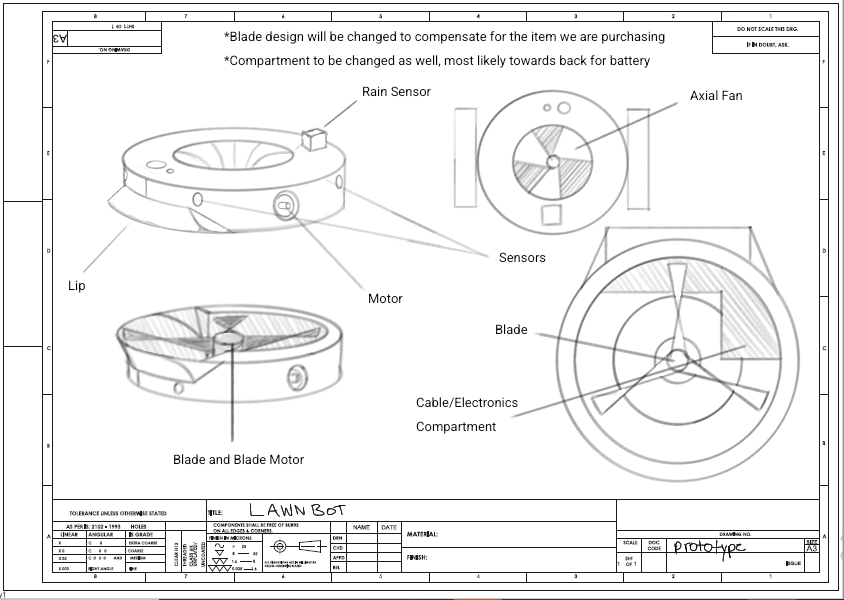
\includegraphics[width = 0.8\textwidth]{root/Lawn_Bot_V1.jpg}
        %\includegraphics[width = 0.2\textwidth]{root/UB-Seal.eps}
        \caption{LawnBot Design (\today)} 
        \label{fig:LawnBot_Design_V1}
    \end{figure}
\end{comment}

\subsection{Testing Phase}
Realizing the material list's delivery date, we purchased a kit to test on, containing a similar microcontroller, to start the software and wiring testing/implementation. This will speed up the process into understanding the automation field of the project and start the testing phase of our project while helping us plan ahead once we get our actual equipment. \par

%\newpage
\section{Software} \label{ch3}
%Introduction Paragraph or two
The software team has begun looking into the coding of our project. With the test kit, we discovered that what was sent is not the same as the microcontroller we plan on using. This is a minor setback as we planned on being able to start coding sooner, but will now need to wait until we have components from our order to begin. For the time being, we have started a GitHub repository in order to track all our changes and collaborate on the coding. \par

\subsection{Algorithm}
We have been looking for the proper algorithm that would work with our project. So far we have found a few that seem to work great with what we want to do but have some cons. As of right now the ones that we have found are Dubins car path planning, Vector field histogram (VFH), A*(A-Star). From what we have read all of these algorithms seem to work great with path finding but the one that seems to be most effective is A* since the others tend to want to follow the shortest path but we want a set path to be followed. We have also started designing and preparing how we want our data base to look like for it to receive the information for the path to follow. \par


\label{EndOfText}
% put this back in if we use End of Text

%\newpage
%\pagenumbering{Roman} 
%\addcontentsline{toc}{section}{List of Figures}
%\fancyfoot[C]{Page \thepage\ of \pageref{endOfDoc}}
%\listoffigures
%\thispagestyle{fancy}

%\newpage
%\addcontentsline{toc}{section}{List of Tables}
% put this back in if we use End of Text
%\listoftables
%\thispagestyle{fancy}

\label{endOfDoc}
\end{document}